\chapter{Neural networks}
Artificial neural networks were originally created as a way of modeling behavior of biological
neurons. However most common use of those models in modern times is not focused on close
replication of biological behavior and instead uses simplified neuron like mathematical 
functions for solving classification and prediction problems.
While some of modern network models still look into nature for an inspiration, like for example
convolutional networks that are inspired by by visual cortex, many of them focus just on 
effectivnes of model and on problem that it tries to solve.
As an example of element unpresent in nature but used frequently in artificial networks a 
rectifier activation function can be given.

%====================================================================================================
\section{History}

%----------------------------------------------------------------------------------------------------
\subsection{Biological inspiration}

\subsubsection{Neuron as a cell}
Neurons are at their core cells so most of metabolic processes common for animal cells also
occur in them. However just like red blood cells neural cells do not divide on their own and new
neurons are generated by specialised stem cells.
\begin{figure}[ht]
	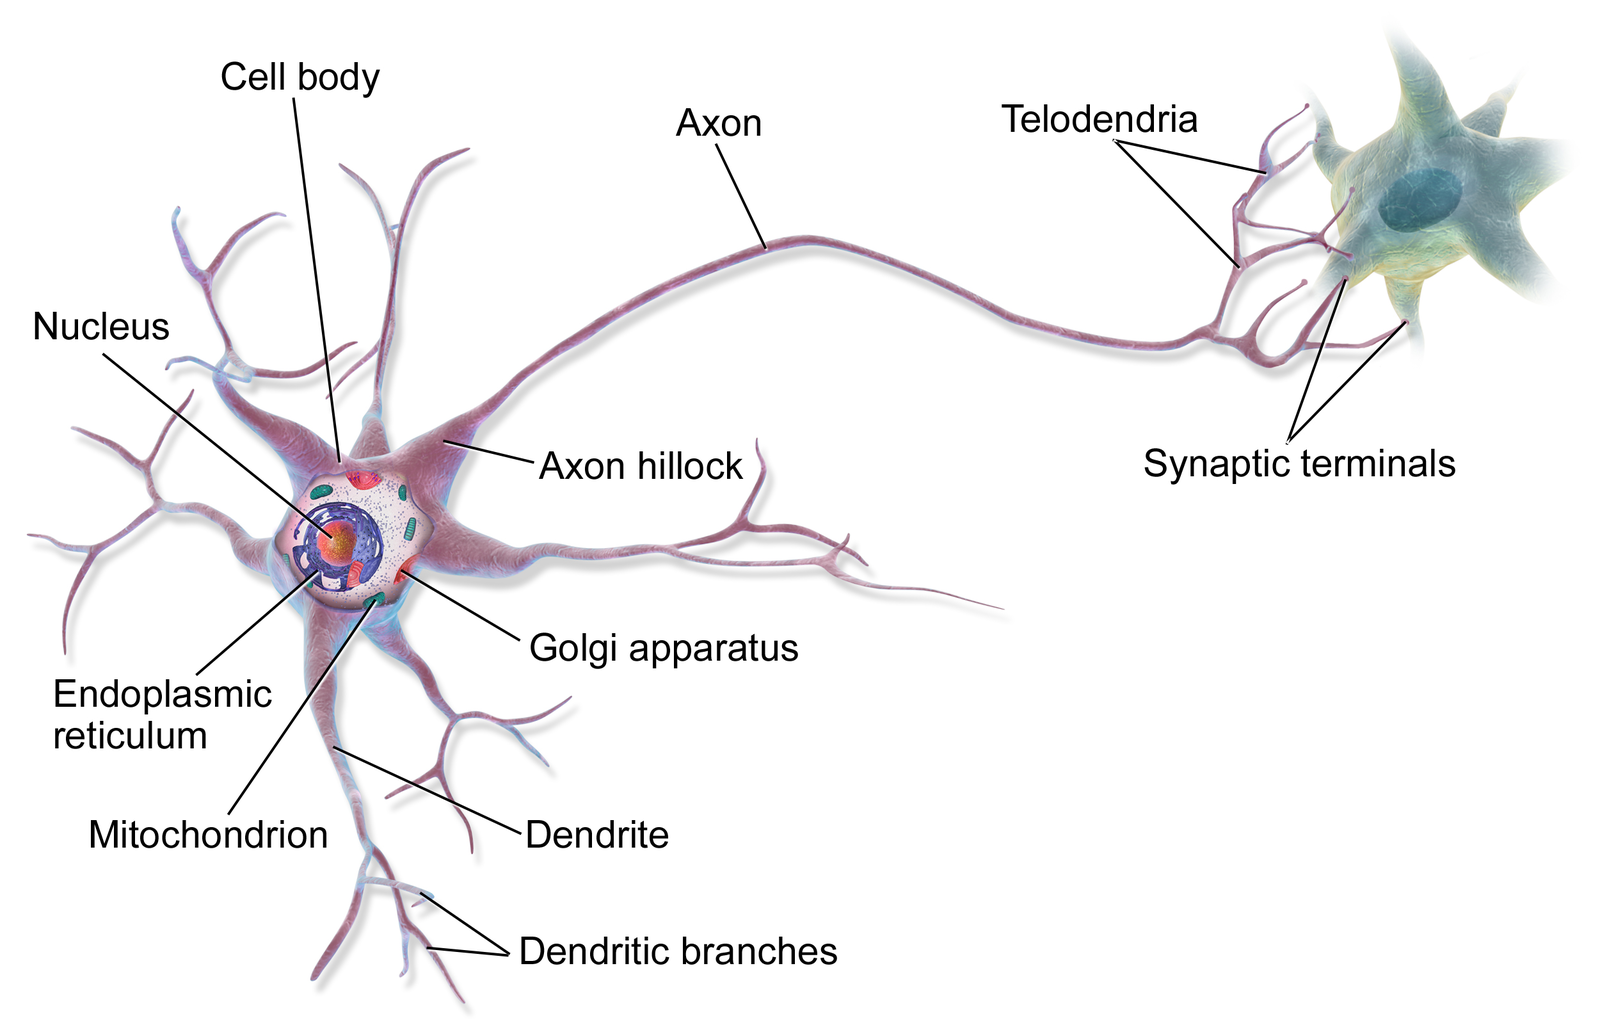
\includegraphics[width=\textwidth]{figures/Blausen_MultipolarNeuron}
	\caption{Neural cell structure. Image by Bruce Blaus}
	\label{fig:Blausen-Neuron}
\end{figure}
There is however one behavior that until recently was believed to be specific to only neural cells
and only recent studies extend this ability to glial cells.
This is ability to transfer a electric signal trough length of cell axon that allows a long range
electrical signal transmision.

\subsubsection{Electrochemicall signal transmission}
Cell body of non activated neuron have a potential of $U_{r}=70mV$ called 
\textit{resting potential}.
This potential is a result of an active biochemical process that removes sodium cations $Na^{+}$
outside of a cell body. Because cell membrane is hardly permeable for soduim ions when in resting
state an electric diffusion is incapable of fully counteracting this process and an equilibrium
is achieved at $U_{r}$.
Signals recieved by a neuron increase its potential

\subsubsection{Naural systems}

%----------------------------------------------------------------------------------------------------
\subsection{Cybernetics, first steps in modeling of neural systems}
The first branch of science that tried do decopule neuron models from its biological basis was 
cybernetics. The term cybernetics originates from greek word \textbf{TODO: GREEK LETTERS} which
originally meant a helmsman. However even Aristotel used it to describe people that control 
other systems then boat. In modern Greek KIBRNETES means either a manager or a control system and 
helmsman is called PEDALIONHOS.
Term cybernetics was first used in its moder meaning by Norbert Wiener in 1948 in book 
``Cybernetics or control and Communication in the Animal and the Machine''. 
In that publication Wiener describes application of technical and mathematical analysis 
that was used for mechanic systems to biological organisms.
\begin{figure}[ht]
	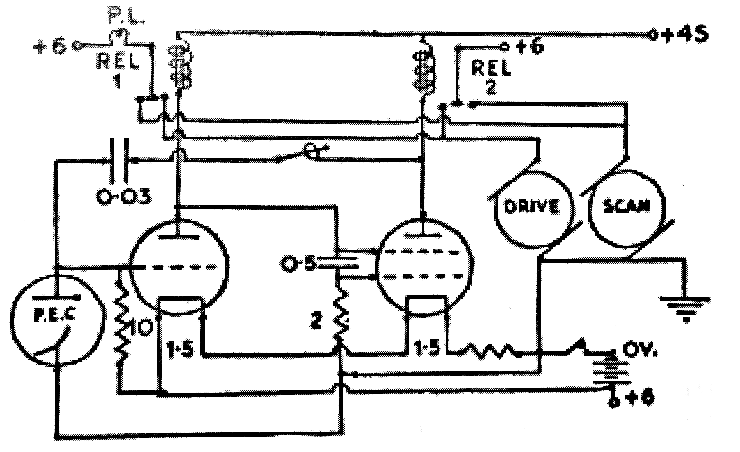
\includegraphics[width=\textwidth]{figures/speculatrix}
	\caption{Machina speculatrix}
	\label{fig:machina_speculatrix}
\end{figure}
Alongside his research Weiner created Machina Speculatrix, a simple robot that attempted to
emulate a behavior of animals with simple neural systems.
% FIXME: ZRZYNKA
The robots used two motors  one for a front-wheel drive, the other for steering, to move around.
The speed of these motors were affected by two different sensors. In low light, 
the robots moved forward and steered slowly. In medium light, the steering motor stopped so
that the robot moved directly towards a light source. 
In bright light, the robot was dazzled, with the steering motor speeding up. 
A similar dazzled state (accompanied by a brief period of complete insensitivity to light)
was entered when the robot shell was bumped by an obstacle.

These robots were of interest because they generated very complex behaviors as a 
function of the interaction between their simple reflexes and a complex world.
They are of renewed interest today because they illustrate many of the principles 
that guide embodied cognitive science. 
% KONIEC ZRZYNKI
\begin{figure}[ht]
	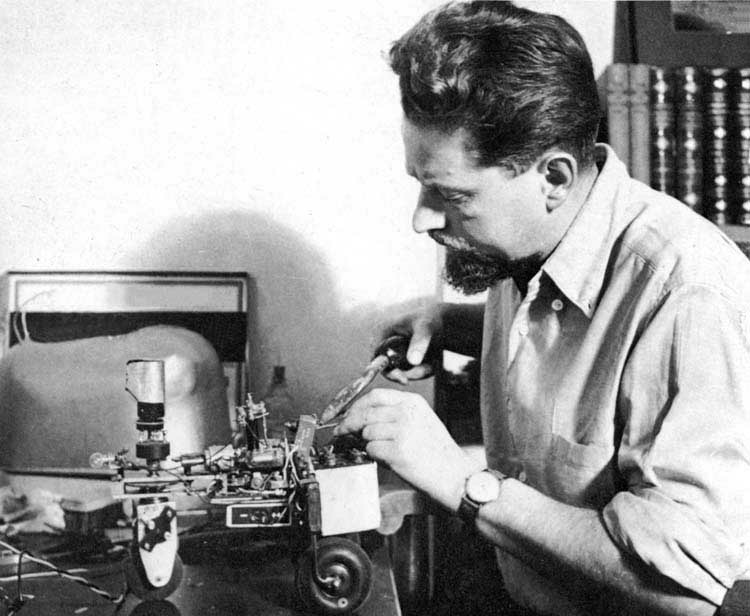
\includegraphics[width=\textwidth]{figures/grey_turtle}
	\caption{Walter Gray and his tortoise (Machina Speculatrix)}
	\label{fig:grey_turtle}
\end{figure}
Later on more complex electrical neuron equivalents were created, one of such models that
was used commonly was one creted by Harmon.
\begin{figure}[ht]
	
\includegraphics[width=\textwidth]{figures/snek}
	\caption{Harmons neuron}
	\label{fig:harmon}
\end{figure}
Those models were capable of recreating a basic behavior of neural cell however most important
influence of cybernetics is system based approach.
In that approach every entity can be modelled as a system that is equivalent of transformation

%====================================================================================================
\section{Feed forward neural networks}

%----------------------------------------------------------------------------------------------------
\subsection{Mathematical model of neuron}
First mathematical model of the neural cell was created in 1943 by Warren MuCulloch and Walter Pitts.
It aimed at recreating an behavior of the neuron electric potenitial activation as a result of
synaptic potential reaching specific bias. What is important this model was never supposed to
precisely mimic behavior of biological neuron and as such do not include representation of metabolic
processes or even neurotransmition.
However despite significant simplification McCulloch-Pitts neuron proven to have many uses and
its basic structure were used to create most of modern day models.
Essentialy in this model neuron is a finction $f_n(x):\mathbb{R} \rightarrow \{ 0,1 \} $ where $n$
is size of input.
In such case equation describing neuron response is as follows:
The basic model of the neuron (neural layer) was created in 1943 by McCullough and Pitts 
\cite{McCulloch1943}. It described response of neural layer to multiple signals with
equation $y= \chi (W\cdot x+b)$, where $y$ is response, $x$ input, $W$ weights, $b$ bias and
$\chi$ is a step function.
Algorithm for automated adjustment of weights in relation to data was proposed in 1958
by Rosenblatt \cite{Rosenblatt58}. This model and all its successors can be described
as an aggregation, dampening, and activation signal path.
\begin{figure}[ht] 
	\centering
	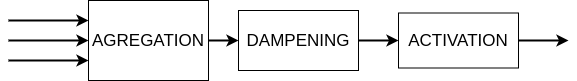
\includegraphics[width=10cm]{figures/basic_neuron}
	\caption{Generalized model of a neuron}
	\label{fig:basic_neuron}
\end{figure}
In the case of McCullough-Pitts neuron aggregation is a weighted sum, dampening is the subtraction
of a bias and activation is a step function. While other models have some differences,
usually different activation functions, the basic signal flow remains unchanged.
While this model and its successors were inspired by a biological neuron there are much
more simplified. One of those simplifications is the lack of time-domain in the model which means
that response of a layer depends only on its current input.
This is in contrast with biological networks that are sensitive not only for a signal value
but also for its change over time.

%----------------------------------------------------------------------------------------------------
\subsection{Perceptron, abilities and limitations}
Simple perceptron is a McCullouch-Pitts neuron with a learnig alorithm assigned to it.
Therfore perceptron equation can be described as a :
\begin{equation}
	y = \chi (W\cdot x+b),
\end{equation}
where $\chi$ is a step function described as:
\begin{equation}
	\chi (x) =  
	\begin{cases}
		1        \quad \text{if } u > 0\\
		0        \quad \text{if } u \leq \\
	\end{cases}
\end{equation}
As perceptron rule is an example of a supervised learning it reqire a training set where for 
each input $x_{j}$ a corresponding expected output $d_{j}$ is provided. 
Then algorithm adjusts weights and bias of given neuron so that it response will 
correspond to expected one. 
Weights and biasa together are considered parameters of neuron and described as a:
\begin{equation}
	\phi = \{ W,b \}.
\end{equation}
\begin{figure}[ht] 
	\centering
	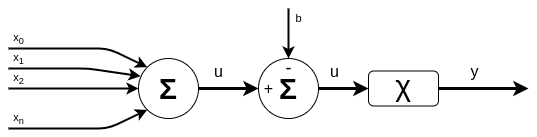
\includegraphics[width=\textwidth]{figures/perceptron}
	\caption{Perceptron}
	\label{fig:perceptron}
\end{figure}
Percetron rules works by excuting following steps:
\begin{itemize}
	\item If value of $y_{j}$ is equal to expected value $d_{j}$ then weights $W$ and 
		  bias $b$ remain unmodified.
	\item If value $y_{j}=0$ and $d_{j}=1$ then weights are to be updated acording to 
		  equation $W:=W+x_{j}$ and bias acording to equation $b:=b+1$.
	\item If value $y_{j}=1$ and $d_{j}=0$ then weights are to be updated acording to 
		  equation $W:=W-x_{j}$ and bias acording to equation $b:=b-1$.
\end{itemize}
After parameter update a new input-output pair is presented and algorithm repeats until all 
pairs from learning set are processed.
Perceptron rule was later generalied into a Widrow-Hoff rule according to which parameters are 
updated as described in equation :
\begin{equation}
	\Delta W_{j} = x_{j}(d_{j}-y_{j}),\\
	\Delta b_{j} = d_{j} - y_{j},\\
	W :=  W + \Delta W_{j},\\
	b := b + \Delta b_{j}.
\end{equation}
If only possible responses of neuron are 0 and 1 then Widrow-Hoff rule behaves exactly like a
perceptron rule.
Aim of lerning is minimalization of energy function of neuron response which is described as a:
\begin{equation}
	E = \sum_{j=0}^{n}(y_{j}-d_{j})^{2}
\end{equation}
Because step function is not continous in point 0 it is impossible to calculate it derivative
an therfore gradient based learing algorithms cannot be used for perceptron.
This limits this model to a single layer nework which is hightly problematic as such network
is very limited in its applications.
One of most basic examples ccan be a inability of perceptron to realize XOR function.
This is because in case of two dimensional input perceptron divides space into two lineary
seperable subspaces.
\begin{figure}[ht] 
	\centering
	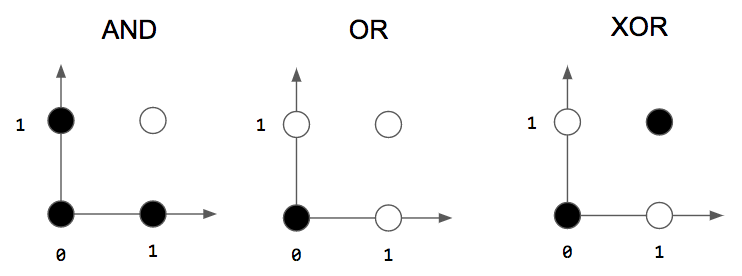
\includegraphics[width=10cm]{figures/logic_neuron}
	\caption{Logic functions presented on 2D space}
	\label{fig:logic_neuron}
\end{figure}
Exculsive alternative do to its nature is not a lineary seperable function. It is however
possible to create a realization of XOR with perceptron like neurons by recreating a logic
circuit that is equivalent to XOR while using only OR, NOT, AND gates.
\begin{figure}[ht] 
	\centering
	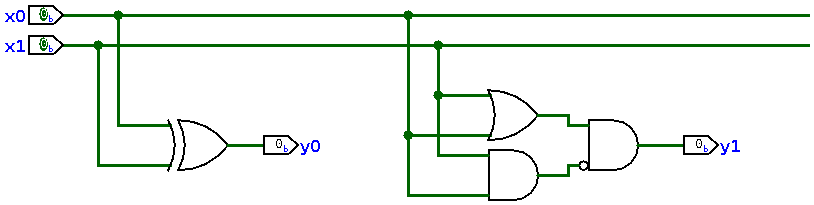
\includegraphics[width=\textwidth]{figures/xor_circ}
	\caption{XOR circuit and it equivalent}
	\label{fig:xor_circ}
\end{figure}
However while such network will process data it cannot learn anything new, to solve that 
problem a new approach must be taken.

%----------------------------------------------------------------------------------------------------
\subsection{Backpropagation and multi layer neural networks}
First succesfull atempt at creating learning algorithm for multilayer neural network was made
in 1986 year by Rumelhart, Hinton and Williams. That algorithm was a backpropagation and as it
requires calcualation of simple gradient underlying activation function must be differentiable.
Because of that step function was repleaced bya logistic function as the neuron activation.
There is a unipolar variant
\begin{equation}
	f_{a}(u) = \sigma(u) = \frac{1}{1+e^{-\beta u}},
\end{equation}
which alongside its bipolar eqiuvalent
\begin{equation}
	f_{a}(u)=tanh(\beta u),
\end{equation}
became most widely used activation functions.
\textbf{TODO:ADD PLOTS FOR VARIOUS BETA VALUES}
Important trait of sigmoidal function is it differenciability. In case of unipolar function
with $\beta = 1$ resulting \textbf{TODO: JAK JEST ROZNICZKA PO ANGIELSKU} is described as a 
\begin{equation}
	\frac{df_{a}(u)}{du}=f_{a}(u)(1-f_{a}(u)).
\end{equation}
In case of bipolar function with $\beta = 1$ result is as follows:
\begin{equation}
	\frac{df_{a}(u)}{du}=1-f_{a}^{2}(u).
\end{equation}
Those functions are trivial to calculate nuerically as all they require is value of a base
function for given input. It is also worth noting that for $\beta \rightarrow \inf$ sigmoidal
functions start to behave like a step function.
Backpropagation is an example of supervised learning where a energy function of te neuron
response is minimmized
\begin{equation}
	E=\frac{(y-d)^{2}}{2}
\end{equation}
With that we can calculate a gradient for a j-th input, desired output pair with an following
equation:
\begin{equation}
	\Delta_{j}E = \frac{\partial E}{\partial W_{j}} = (y_{j}-d_{j})x_{j}\frac{df_{a}(u_{j})}{du_{j}}. 
\end{equation}
For conviniece it is reasonable to write a part related to neuron response as a:
\begin{equation}
	\delta_{j} = (y_{j}-d_{j})\frac{df_{a}(u_{j})}{du_{j}}, 
\end{equation}
so that discreete weight update function can be written as a 
\begin{equation}
	W := W - \eta \delta_{j} x_{j},
\end{equation}
where $x_{j}$ is related to network input,  $\delta_{j}$ to output and $\eta \in <0,1>$ is a 
constant learning factor.
Learning factor is considered a metaparameter and is set once for whole learning process, 
therfore a seto of metaparameters for simple backporbagation algortihm can be described as 
a $\Phi = \{\eta \}$. There is also a continous approach to adjusting network parameters that
relies on solving differencial equation
\begin{equation}
	\frac{dW_{j}}{dt} = -\mu \delta_{j} x_{j},
\end{equation}
where $\mu$ is equivalent of $\eta$ from discrete model. However as this work focuses on 
numerical solutions a discrete model was chosen and no more attention will be given to a 
continous one.
Choice of correct learning rate is crucial in designing a efficen backpropagation 
learning algorithm as two small value can result in slow convergence rate and high risk of 
getting stuck in local minima. On the other hand high learning rate may result in algorithm
jumping over desired solution and never converging on it. 
\begin{figure}[ht] 
	\centering
	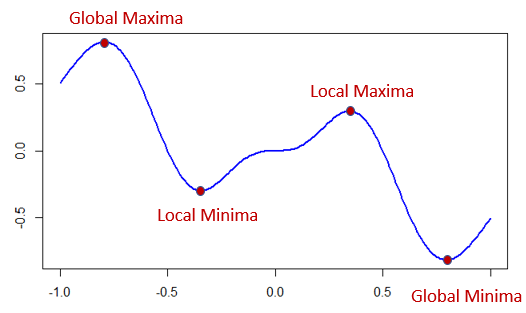
\includegraphics[width=\textwidth]{figures/local_minima}
	\caption{Example of local and global minima}
	\label{fig:local_minima}
\end{figure}

%----------------------------------------------------------------------------------------------------
\subsection{Other gradient based optimalizators}
As effient as it is in solving simplier problems basic gradient descent have to many limitations,
over the years many extensions of that algorithm were created.

\subsubsection{Momentum}
Simpliest modification of gradient descent that can counteract problem with getting stuck in 
local minima is addition of momentum. 
Momentum, denoted as $\alpha \in <0,1>$, is used in order to influence learning algorithm 
parameter adjustment values in current step by its values from pervious steps.
This mimics momentum from physics where body with some mass that was put in motion by external
force will not stop immidietly if this force is removed.
In this approach change of weights for input-output pair $j$ denoted as $\Delta W_{j}$ is 
described by an equation:
\begin{equation}
	\Delta W_{j} = -\eta \delta_{j} x_{j} + \alpha \Delta W_{j-1}.
\end{equation}
For initial pair $j=0$ the momentum component $\Delta W_{j-1}$ is set to zero as gradient 
descent starts from standstill.
Choice of correct value for hyperparameter $\alpha$ depends on specific training data.
If there are a lot of plateaus or large nuber of local minimas a larger momentum must be set
otherwise algorithm will get stuck. On the other hand if a very narrow solution is expected
a small value of momentum is preffered otherwise algorithm will jump over optimal solution and
never find it. \textbf{TODO: IMAGE OF PLATEAUS AND LOCAL MINIMAS}.
One of approaches that allows more freedom in setting momentum factor is to check for change of
energy function after weight adjustement. If increase of enrfy function is by less
of a given factor $\beta$ then that weight adjustemnt is accepted otherwise it is recalculedet
with $\alpha$ set to zero. 

\subsubsection{Nesterov}
Momentu based optiization was enchanced by Yuri Nesterov in 1983 by presenting a accelerated
momentum based gradient optimizer. This approach introduces only one change, network response
is calculated using not current weights and bias but one updated with momentum only.
\begin{equation}
	\bar{y} = f_{a}((W+))	
\end{equation}


\subsubsection{AdaGrad}

\subsubsection{RMSProp}

\subsubsection{Adam}

%----------------------------------------------------------------------------------------------------
\subsection{Limitations on neural networks depth}


%====================================================================================================
\section{Recurrent networks and deep learning}

%----------------------------------------------------------------------------------------------------
\subsection{Deep learning models}
\subsubsection{Activation functions for deep networks}
\subsubsection{Vector processing unit}
\subsubsection{Types of deep networks}

%----------------------------------------------------------------------------------------------------
\subsection{Simple recurrent networks}
Simple solution to problem of time independence is to concatenate response of neural layer
from previous cycle to it input $x'(t)=[x(t)|y(t-1)]$.
Such solution results in signal propagating trough time and influencing responses of future cycles,
if this is the only modification to the feed-forward model such layer is called Simple Recurrent
Unit (SRU).
\begin{figure}[ht] 
	\centering
	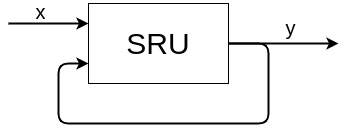
\includegraphics[width=5cm]{figures/sru}
	\caption{Simple Reccurent Unit (SRU)}
	\label{fig:sru}
\end{figure}
While this solution makes model time aware it has its own problems, mainly a signal vanishing
issue. Since the input signal from a cycle, $n$ has direct influence only on a response of this
cycle and for each subsequent cycle, it is the only through a feedback loop.
Influence of input $n$ on response of cycle $n+k$ grows inverse proportional to $k$.
This means that in this model only those regularities that appear over short time periods can
be detected.
Making weights on feedback bigger will not eliminate the problem and instead replace it with signal
an explosion that causes a response to reach maximum value if a strong signal appeared on input at
least once.

%----------------------------------------------------------------------------------------------------
\subsection{Long short term memory networks}
\subsubsection{LSTM unit model}
One of the possible solutions to this issue is the addition of long term memory which will regulate
forward and loopback path influence on neuron response, such a solution is used in long short
term memory (LSTM) networks \cite{Hochreiter1997}.
% TODO: Move legend below, write more precisely about neuron and no neurn
\begin{figure}[ht] 
	\centering
	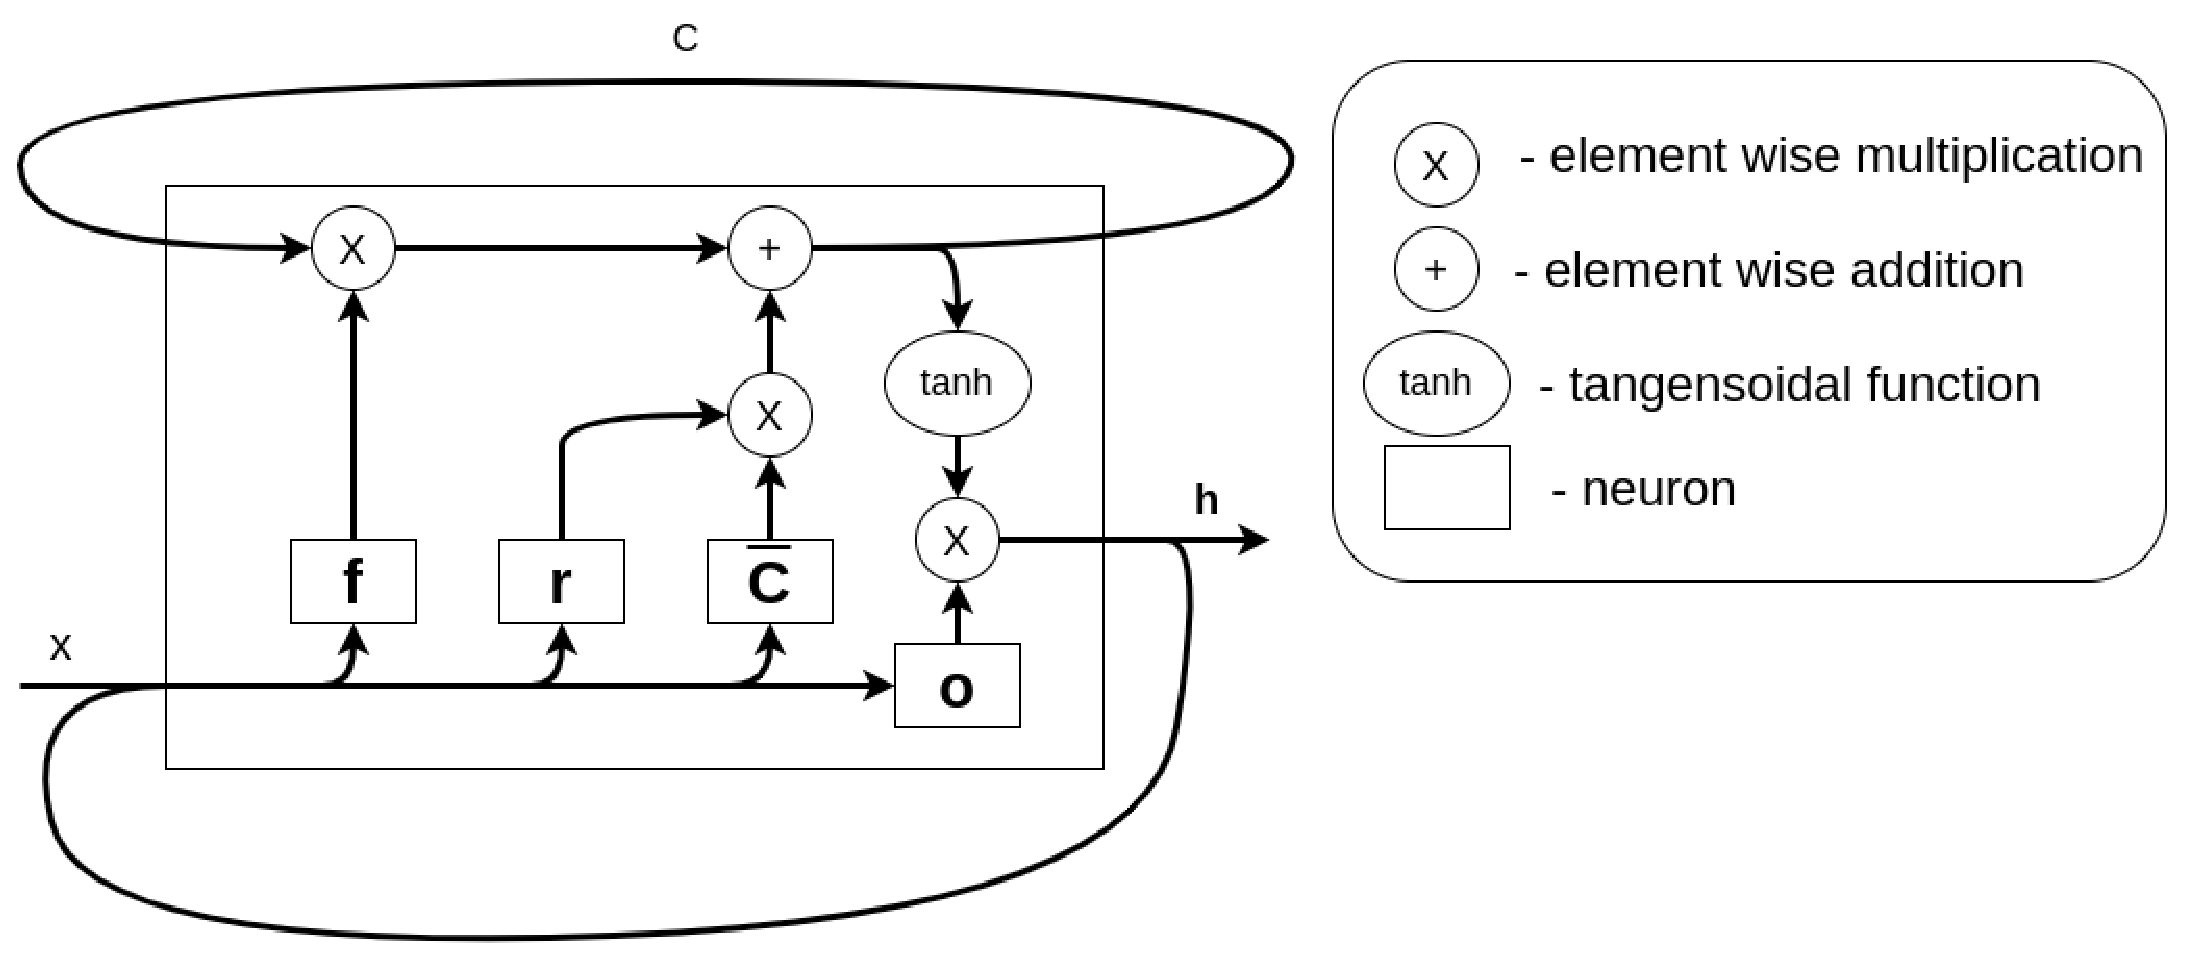
\includegraphics[width=\textwidth]{figures/lstm}
	\caption{LSTM layer}
	\label{fig:lstm}
\end{figure}
Single LSTM neuron consists of four basic neurons and two non-neuron operations:
\begin{itemize}
	\item $x'(t)=[x(t)|h(t-1)]$,
	\item $o_t=\sigma (W_o x'_t+b_o)$,
	\item $r_t=\sigma (W_r x'_t+b_r)$,
	\item $f_t=\sigma (W_f x'_t+b_f)$,
	\item $\bar{C}_t=\tanh (W_c x'_t+b_c)$,
	\item $C_t=f_t\odot C_{t-1}+r_t\odot \bar{C}_t$,
	\item $h_t=o_t\odot \tanh (C_t)$,
\end{itemize}
with $W$ and $b$ being weights and biases for each basic neuron, $x$ input, $y$ output and
$C$ long term memory. As can be seen, $o_t$ is the equivalent of SRU and is moderated by
long term memory before propagating as output. Temporary value of long term memory based
only on current output $\bar{C}_t$ is calculated and then with help of neurons $r$ and $f$
is transformed into its final value.
Neuron $r$ is called remembering gate and influences to what degree temporary long term
a memory from a given cycle affects its final value while $f$ is forgetting gate and
decides the influence of long-term memory from the last cycle on the current one.
Thanks to such implementation our model can learn to detect both long term regularities and 
short term ones.

\subsubsection{Backpropagation through time}

